% Created 2018-11-08 Thu 02:52
% Intended LaTeX compiler: pdflatex
\documentclass[11pt]{article}
\usepackage[utf8]{inputenc}
\usepackage[T1]{fontenc}
\usepackage{graphicx}
\usepackage{grffile}
\usepackage{longtable}
\usepackage{wrapfig}
\usepackage{rotating}
\usepackage[normalem]{ulem}
\usepackage{amsmath}
\usepackage{textcomp}
\usepackage{amssymb}
\usepackage{capt-of}
\usepackage{hyperref}
\usepackage{minted}
\usepackage[a4paper, margin=2cm]{geometry}
\usepackage{indentfirst}
\usepackage[, brazilian]{babel}
\usepackage[bottom]{footmisc}
\usepackage{float}
\usepackage{subcaption}
\usepackage{titling}
\setlength{\droptitle}{-1.5cm}
\hypersetup{ colorlinks = true, urlcolor = blue }
\date{\today}
\title{}
\hypersetup{
 pdfauthor={},
 pdftitle={},
 pdfkeywords={},
 pdfsubject={},
 pdfcreator={Emacs 26.1 (Org mode 9.1.14)}, 
 pdflang={Brazilian}}
\begin{document}

\begin{titlepage}
	\begin{center}
		\Huge{Universidade Federal de Minas Gerais}\\
		\vspace{15pt}
    \Large{Reuso de Software}\\
    \vspace{95pt}
    \textbf{\LARGE{Trabalho Prático}}\\
		%\title{{\large{Título}}}
		\vspace{3,5cm}
    \begin{figure}[h]
      \begin{center}
        
\includegraphics[scale = 0.50]{img/ufmg-logo.png}
      \end{center}
     \label{fig:graph}
    \end{figure}
	\end{center}
  \begin{flushleft}
		\begin{tabbing}
        \textbf{Grupo 2:}\\
        Daniel Cruz \\
			  Fernanda Guimarães \\
        Gabriel Bastos \\
        Lucas Furtini \\
        Manoel Júnior
	    \end{tabbing}
  \end{flushleft}
	\vspace{1cm} 
	\begin{center}
		\vspace{\fill}
		Novembro\\
		2018
	\end{center}
\end{titlepage}
\section{Introdução}
\label{sec:org5f82a3e}
O tema do trabalho são jogos para Simulação de Engenharia de Software. O grupo reusou e
reutilizou o projeto do SimulES no github. Além da refatoração do código existente,
foram adicionadas novas \emph{features}, tornando o projeto de fato uma linha de produtos de
\emph{software}.
\section{Linha de Produtos de \emph{Software} (SPL)}
\label{sec:org038cc19}
\begin{figure}[H]
\centering
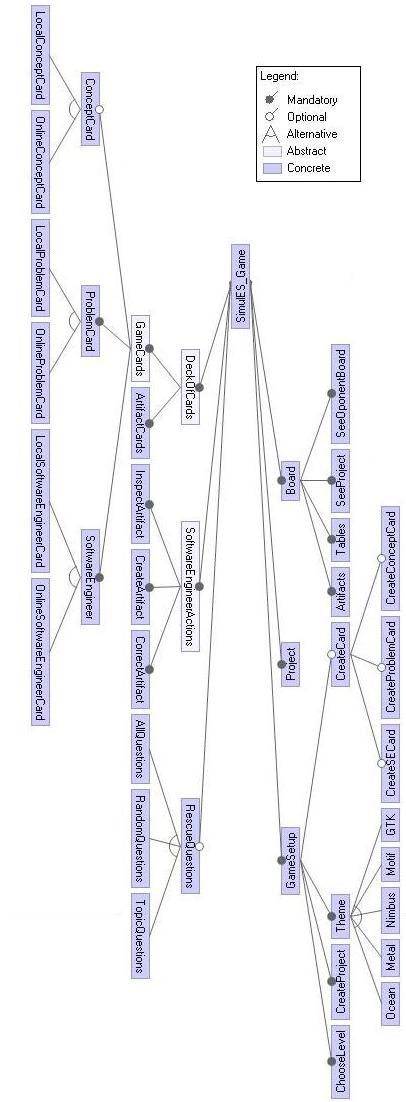
\includegraphics[height=580px]{./img/features.jpeg}
\caption{diagrama de características.}
\end{figure} 
\subsection{Look'n Feel}
\label{sec:orgbfc4934}
Para que o jogo possa de adequar à diversos temas, foram adicionadas cinco opções de
\emph{look'n feel}\footnote{\href{https://pt.wikipedia.org/wiki/Look\_and\_Feel}{Look'n Feel}}:
\begin{figure*}[h] \centering
\begin{subfigure}[t]{0.33\textwidth} \centering
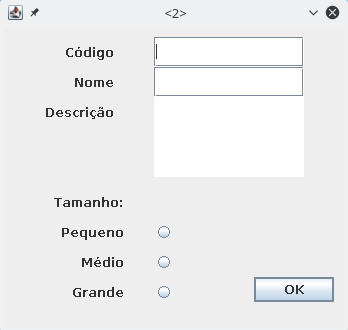
\includegraphics[height=150px]{./img/ocean.png}
\captionsetup{labelformat=empty} \caption{Ocean}
\end{subfigure}
\begin{subfigure}[t]{0.33\textwidth} \centering
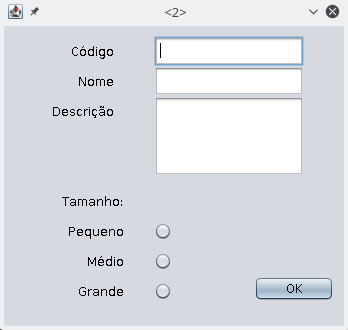
\includegraphics[height=150px]{./img/nimbus.png}
\captionsetup{labelformat=empty} \caption{Nimbus}
\end{subfigure}
\begin{subfigure}[t]{0.32\textwidth} \centering
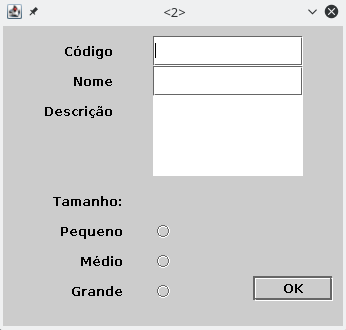
\includegraphics[height=150px]{./img/metal.png}
\captionsetup{labelformat=empty} \caption{Metal}
\end{subfigure}
\end{figure*}
\begin{figure*}[h] \centering
\begin{subfigure}[t]{0.35\textwidth} \centering
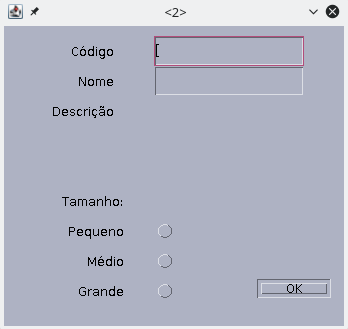
\includegraphics[height=150px]{./img/motif.png}
\captionsetup{labelformat=empty} \caption{Motif}
\end{subfigure}
\begin{subfigure}[t]{0.35\textwidth} \centering
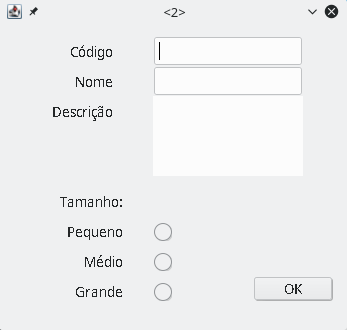
\includegraphics[height=150px]{./img/gtk.png}
\captionsetup{labelformat=empty} \caption{GTK}
\end{subfigure}
\end{figure*}
\subsection{Questão de Resgate}
\label{sec:org94755c7}
A questão de resgate é um artifício de balanceamento baseeado na Teoria dos Jogos. Ela
serve para permitir a recuperação de jogadores em situações complicadas. Assim,
estende o jogo com uma nova dinâmica de perguntas e respostas.

Sua configuração possui definição de 3 estratégias de construção do banco de questões:
todas as questões, questões aleatórias, e questões de um certo tópico, como por
exemplo, arquitetura de \emph{software}.

Já a regra de uso da questão de resgate é muito simples: o jogador que não possuir
nenhuma carta em mãos e tirar 1 no dado, terá a chance de responder uma questão de
resgate. Caso acerte, irá sacar o número máximo de cartas (5).
\begin{center}
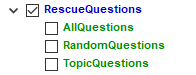
\includegraphics[height=0.12\textwidth]{./img/unchosen.png}
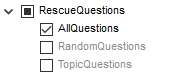
\includegraphics[height=0.12\textwidth]{./img/chosen.png}
\end{center}
\begin{figure}[H]
\centering
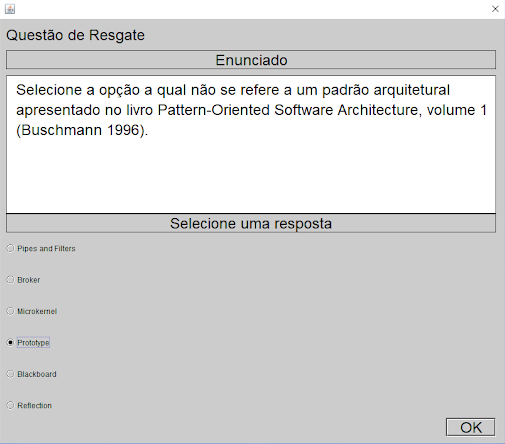
\includegraphics[height=250px]{./img/question.png}
\caption{questão de resgate.}
\end{figure} 
\subsection{Criação de cartas}
\label{sec:orgd6be45d}
Para a criação de novas cartas, implementamos estas opções no menu principal, além das
respectivas telas para a entrada dos dados da carta.
\begin{figure*}[h] \centering
\begin{subfigure}[t]{0.45\textwidth} \centering
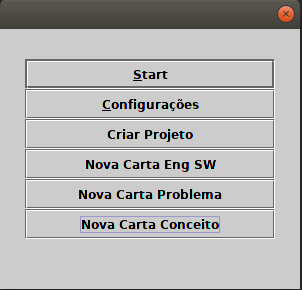
\includegraphics[height=150px]{./img/start.png}
\captionsetup{labelformat=empty} \caption{Menu principal.}
\end{subfigure}
\begin{subfigure}[t]{0.45\textwidth} \centering
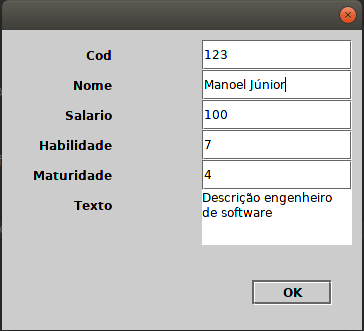
\includegraphics[height=150px]{./img/mcard.png}
\captionsetup{labelformat=empty} \caption{Tela de criação de engenheiro de \textit{software}.}
\end{subfigure}
\end{figure*}
\begin{figure}[H]
\centering
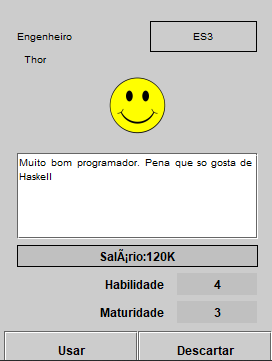
\includegraphics[height=160px]{./img/ccard.png}
\caption{carta criada.}
\end{figure} 
\subsection{Compartilhamento de cartas}
\label{sec:orgac9cd0a}
Para a \emph{feature} de cartas compartilhadas, utilizamos como hospedagem para o
repositório de cartas o serviço \emph{Amazon AWS}. O repositório é aberto para
contribuição. Já o compartilhamento, sendo efetivamente uma \emph{feature}, é configurável
por tipo de carta:
\begin{itemize}
\item Conceito
\item Problema
\item Engenheiro de \emph{software}
\end{itemize}
\begin{figure*}[h] \centering
\begin{subfigure}[t]{0.45\textwidth} \centering
\begin{center}
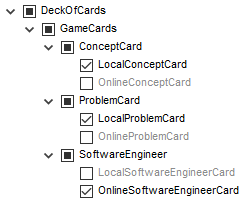
\includegraphics[height=110px]{./img/config.png}
\end{center} 
\captionsetup{labelformat=empty} \caption{configuração da \textit{feature}.}
\end{subfigure}
\begin{subfigure}[t]{0.45\textwidth} \centering
\begin{center}
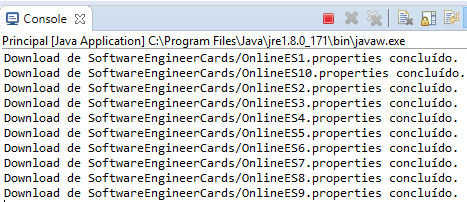
\includegraphics[height=85px]{./img/download.png}
\end{center} 
\captionsetup{labelformat=empty} \caption{Log de download das cartas.}
\end{subfigure}
\end{figure*}
\section{Aspecto de Logging}
\label{sec:org4ff6012}
O código de logging estava espalhado através de várias partes do código. Havia dois
problemas típicos: \emph{tangling} e \emph{scattering}.  Para resolver tais problemas, foi criado
o aspecto de \emph{logging}.
\begin{figure}[H]
\centering
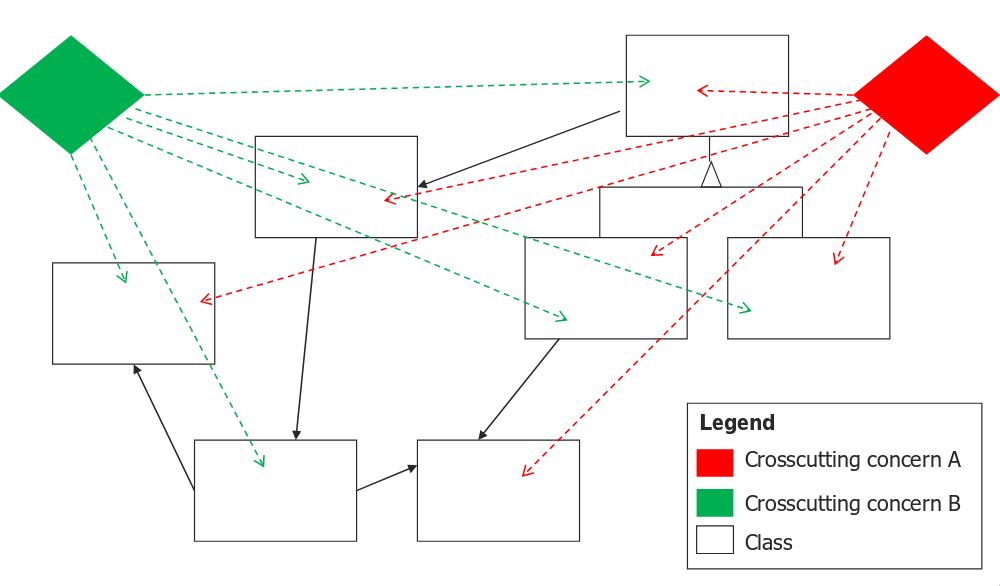
\includegraphics[height=160px]{./img/solution.png}
\caption{solução com aspectos.}
\end{figure} 
O aspecto de logging, como o nome já diz, é um aspecto que reúne todos o código de
\emph{logging} do jogo em um módulo, o \emph{LoggingAspect.aj}. Assim, isto resolve os problemas
citados anteriormente.
\pagebreak
\section{Padrão Arquitetural}
\label{sec:org8e10a82}
O padrão arquitetural do SimuLES é o de três camadas (layers). É muito utilizado em
sistemas com interface:
\begin{itemize}
\item Facilita o desenvolvimento incremental.
\item Facilita o reuso.
\item Mudanças só impactam camada superior.
\item Utilizada no projeto original.
\end{itemize}
\begin{figure}[H]
\centering
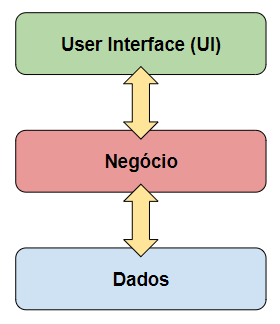
\includegraphics[height=130px]{./img/layers.png}
\caption{diagrama de três camadas.}
\end{figure} 
\section{Padrões de Projeto}
\label{sec:org4fa2e66}
Foram utilizados dois padrões de projeto:
\begin{itemize}
\item Builder\footnote{\href{https://www.geeksforgeeks.org/builder-design-pattern/}{Builder design pattern}}
\item Factory Method\footnote{\href{https://www.tutorialspoint.com/design\_pattern/factory\_pattern.htm}{Factory design pattern}}
\end{itemize}
Builder é um padrão de projeto de \emph{software} criacional que permite a separação da
construção de um objeto complexo da sua representação, de forma que o mesmo processo de
construção possa criar diferentes representações.   

Utilizamos este padrão para garantir flexibilidade na construção do cliente responsável
pelo acesso ao S3 Bucket, recurso empregado na \emph{feature} Cartas compartilhadas.
\begin{figure}[H]
\centering

\includegraphics[height=130px]{./img/builder.png}
\caption{diagrama de classes do Builder.}
\end{figure} 
\pagebreak
O padrão de projeto factory method, sendo também criacional, é um dos mais usados em
Java. Ele permite a criação de um objeto sem expor a criação lógica para o cliente, e
refere-se ao novo objeto usando uma interface comum.
\begin{figure}[H]
\centering

\includegraphics[height=130px]{./img/factory.png}
\caption{diagrama de classes do Factory Method.}
\end{figure} 
\section{Plano de Atividades}
\label{sec:org1bff7c0}
\begin{center}
\begin{tabular}{lrl}
Atividade & \emph{Deadline} & Resposáveis\\
\hline
\emph{Brainstorm} sobre o jogo & 2018-09-12 & Gabriel, Fernanda, Daniel, Manoel, Lucas\\
Reunião de \emph{Kick}-\emph{off} do projeto & 2018-09-26 & Gabriel, Fernanda, Daniel, Manoel, Lucas\\
Definição dos objetivos da SPL & 2018-10-04 & Daniel\\
Definição das técnicas de reuso & 2018-10-15 & Fernanda, Gabriel\\
\emph{Design} da solução & 2018-10-22 & Daniel, Lucas, Manoel\\
Análise arquitetural & 2018-10-23 & Lucas\\
\emph{Design} da \emph{feature} Look'n Feel & 2018-10-26 & Gabriel\\
\emph{Design} da \emph{feature} Repositório de cartas & 2018-10-28 & Daniel\\
Implementação dos \emph{Look'n Feels} & 2018-11-01 & Gabriel\\
\emph{Design} da \emph{feature} Questão de resgate & 2018-11-01 & Daniel\\
\emph{Design} da \emph{feature} Criação de cartas & 2018-11-02 & Manoel, Fernanda\\
Configuração da solução/projeto & 2018-11-03 & Daniel, Fernanda\\
Implementação do Repositório de cartas & 2018-11-03 & Daniel\\
Refatoração do \emph{logging} em aspecto & 2018-11-03 & Fernanda\\
Atualização do \emph{Readme} para o projeto & 2018-11-03 & Gabriel, Daniel\\
Implementação da Questão de resgate & 2018-11-04 & Daniel\\
Elaboração da apresentação & 2018-11-04 & Fernanda, Gabriel, Daniel, Lucas, Manoel\\
Implementação da Criação de cartas & 2018-11-05 & Manoel, Gabriel\\
Apresentação & 2015-11-05 & Fernanda, Gabriel, Daniel, Lucas, Manoel\\
Elaboração da documentação & 2018-11-08 & Fernanda, Gabriel, Daniel\\
\end{tabular}
\end{center}
\end{document}
